\documentclass{article}

\usepackage{amsmath}
\usepackage{amssymb}
\usepackage{mathtools}
\usepackage{fullpage}
\usepackage{enumerate}
\usepackage{graphicx}

\title{Computer Science 577 Notes \\ Machine Learning}
\author{Mendel C. Mayr}
\date{\today}

\begin{document}
	\maketitle
	\vspace{10pt}
	\begin{center}
		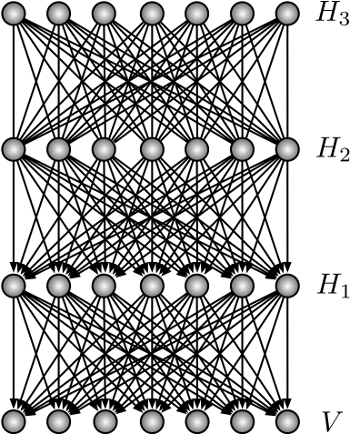
\includegraphics[width = 2.9in]{ann.png}
		\end{center}
	\vspace{16pt}
	\tableofcontents
	\clearpage

	\section{Decision Tree Learning}
		Information gain is used to determine the (feature to) split \\
		Information theory: entropy and information gain:
		\begin{enumerate}[(i)]
			\item Entropy $= H(X) = -\sum_{x \in X}P(X = x)\log_2 P(X = x)$
			\item Conditional entropy $= H(Y|X) = -\sum_{x \in X}P(Y|X = x)$, where \\
			$H(Y|X = x) = \sum_{y \ in Y}P(Y = y|X = x)\log_2 P(Y = y|X = x)$
			\item Mutual information (information gain) $= I(X, Y) = H(Y) - H(Y|X)$
			\end{enumerate}
		Alternative metric: Gini coefficient, i.e. product of probabilities for each of (2) outcomes for the feature \\
		\\
		Limitation of information gain: biased toward tests with many outcomes (i.e. features with many possible values) \\
		C4.5 uses gain ratio: $SplitInfo(D, S) = -\sum_{k \in S} |D_k|/|D| log_2(D_k/D)$, and $GainRatio = I(D, S)/SplitInfo(D, S)$ \\
		\\
		Overfitting: $h \in H$ overfits the training data $D$ if there is an alternative model $h' \in H$ such that $error(h) > error(h')$ yet $error_D(h) < error_D(h)$ \\
		Avoiding overfitting in decision tree learning:
		\begin{enumerate}[(i)]
			\item Early stopping: stop if further splitting not justified by statistical test
			\item Post-pruning: grow large tree, then prune nodes using tuning set \\
			Iteratively eliminate nodes until further reductions reduce accuracy
			\end{enumerate}
		Lookahead: instead of evaluating using information gain, look ahead to see what splits at the next level would be, and measure information gain at a deeper level \\
		\\
		Continuous features: use threshold-based boolean attribute, treshold determined by sorting examples according to the featurem and generating candidate thresholds between adjacent examples with different class values \\
		Threshold chosen from candidates based on information gain \\
		\\
		Training examples with missing attribute values: possible strategies
		\begin{enumerate}[(i)]
			\item At node $n$, upon encountering a missing feature value, assign it the value most common among examples at node $n$, or most common among examples at the node $n$ that also have the same class value
			\item Assign fractional value to attribute for the example and pass fractional example to children for purposes of evaluating information gain
			\end{enumerate}
		\clearpage

	\section{Instance-Based Learning}
		$k$-nearest neighbor classification: given an instance $x_q$ to classify, find $k$ training-set instances that are most simimlar or $x_q$ \\
		Return the class value: $\hat{y} = argmax_{v \in values(Y)} \sum_{i = 1}^k \delta(v, y_i)$ \\
		Various determinations of distance: 
		\begin{enumerate}[(i)]
			\item Hamming distance: number of features with differing values
			\item Euclidean distance: $\delta(x_i, x_j) = \sqrt{\sum_f ({x_i}_f - {x_j}_f)^2}$
			\item Manhattan distance: $\delta(x_i, x_j) = \sum_f ({x_i}_f - {x_j}_f)^2$
			\end{enumerate}
		$k$-nearest neighbor regression: given an instance $x_q$, find the $k$ nearest training-set instances and return $\sum_{i = 1}^k \delta(v, y_i)$ \\
		Distance-weighted nearest neighbor: instances contribute to prediction according to their distance from $x_q$ \\
		\\
		$k$-nearest neighbor does almost nothing at training time, and offsets costs to classification/prediction time \\
		Strategies to speed up $k$-nearest neighbor
		\begin{enumerate}[(i)]
			\item Don't retain every training instance: edited nearest neighbor \\
			Select subset of instances that still provide accurate classifications: \\
			\begin{enumerate}[(a)]
				\item Incremental deletion: delete from memory all training instances redundant to classification
				\item Incremental growth: if training instances insufficient to classify training instance, add to memory
				\end{enumerate}
			\item Use data structure to look up nearest neighbors ($k$-$d$ tree)
			\end{enumerate}
		$k$-$d$ trees ($A^*$ instance search): each node stores one instance, and splits on the median value of the feature having the highest variance \\
		Nodes are pushed to the $A^*$ priority queue with the value indicating the minimum possible distance to the query based on the threshold for the split \\
		\\
		Strenghts of instance based learning: simple, efficeint training, easily adapts to on-line nearning, rubust to noisy data, etc. \\
		Limitations: sensitive to range of feature values, senstivie to irrelevant and correlated features, inefficient classification, no insight into problem domain (i.e. lacks modeling of problem)
		\clearpage

	\section{Probability and Bayesian Learning}
		\subsection{Probabilistic Machine Learning Concepts}
			Recall Bayes theorem: $P(A|B) = P(B|A)P(A)/P(B)$ \\
			\\
			Brute-force MAP learning algorithm:
			\begin{enumerate}[(i)]
				\item Given information $D$, for each hypothesis $h \in H$, calculate the posterior probability $P(h|D) = P(D|h)P(h)/P(D)$
				\item Output hypothesis $h_{MAP}$ with highest posterior probability $h_{MAP} = argmax_{h \in H} P(h|D)$
				\end{enumerate}
			Other probabalisitic concepts in machine learning:
			\begin{enumerate}[(i)]
				\item Maximum likelihood and least-squared error hypotheses
				\item Maximum likelihood hypotheses for predicting probabilities
				\item Minimum description length principle
				\item Bayes optimal classification: $argmax_{v_j \in V}\sum_{h_i \in H} P(v_j|h_i)P(h_i|D)$
				\item Gibb's Algorithm: choose hypothesis $h \in H$ at random, according to posterior probaiblity distribution over $H$, and use $h$ to predict the classification of the next instance $x$ 
				\end{enumerate}
		\subsection{Bayesian networks}
			A Bayesian network consists of a directed acyclic graph and a set of conditional probability distributions \\
			In the each Directed Acyclic Graph (DAG):
			\begin{enumerate}[(i)]
				\item Each node denotes a random variable
				\item An edge from $X$ to $Y$ represents that $X$ directly influences $Y$
				\item Each node $X$ contains a conditional probability distribution representing $P(X|Parents(X))$
				\item Each variable $X$ is independent of its non-descendants given its parents
				\item Each variable $X$ is independent of all others given its Markov blanket
				\end{enumerate}
			Advantages of Bayesian network representation:
			\begin{enumerate}[(i)]
				\item Captures indepdendence and conditional indpendence where they exist
				\item Encodes the relevant  portion fo the full joint distribution
				\item Graphical representation gives insight into complexity of inference
				\end{enumerate}
			Inference task: given values for some variables in the network (evidence) and set of query variables, compute posterior distribution over query variables \\
			Hidden variables: neither evidence nor the query variables \\
			Baysean networks allow for any set to be evidence and any set to be query \\
			Inference by enumeration: consider the chain rule $P(x_1, ..., x_n) = P(x_1)P(x_2|x_1)P(x_3|x_2, x_1)...P(x_n|x_{n-1}, ..., x_1)$ \\
			Posterior probability on query variables can be found via independence, chain rule, and marginalization \\
			\\
			Parameter learning task: given set of training instances and graph structure, infer parameter of conditional probability distributions \\
			Strcture learning task: given set of training instances, infer graph structure (and possibly parameters of CPDs) \\
			For parameter learning, use maximum a posteriori (MAP) estimation: e.g. m-estimates $P(X = x) = (n_x + p_xm)/(\sum_{v \in Values(X)} n_v) + m$, where $p_x$ is prior probability of value $x$, $m$ is number of virtual instances, and $n_v$ is number of occurences of value $v$ 
		\subsection{Expectation Maximization}
			Missing data (hidden variables, values missing at random): values can be imputed using Expectation Maximization (EM) \\
			Iterate until convergence:
			\begin{enumerate}[(i)]
				\item Expectation step: using current model, compute expectation over missing values (missing temporarily take expected values)
				\item Maximization step: update model parameters with those that maximize probability of data (MLE or MAP)
				\end{enumerate}
			Note that $k$-means unsupervised clustering is a form of expectation maximization \\
			Expectation maximation can be hard (takes most likely value) or soft (expectation is probabiltiy distribution) \\
			\\
			Expectation maximation for parameter learning:
			\begin{enumerate}[(i)]
				\item Expecation step: compute probability of each completion of incomplete data points, i.e. answering query over missing variables given others
				\item Maximization step: use completed data set to update Dirchlet distributions, except counts can be fractional, update conditional probability tables
				\end{enumerate}
			Subtelty for parameter learning: overcounting based on number of iterations required to converge to settings for missing values. After each expectation step, reset Dirichlet distributions before repeating maximization step \\
			\\
			Problems with expectation maximization: only finds local optimum, deterministic with respect to priors
		\subsection{Learning Network Structure}
			Chow-Liu algorithm: learns tree structure that maximizes likelihood of training data
			\begin{enumerate}[(i)]
				\item Compute weight $I(X_i, X_j)$ of each possible edge $(X_i, X_j)$
				\item Find maximum-weight spanning tree: use mutual information to calculate \\
				$I(X, Y) = \sum_{x \in values{X}}\sum_{y \in values{Y}} P(x, y)\log_2 P(x, y)/(P(X)P(Y))$ \\
				Prim's algorithm (given $(V, E)$):
				\begin{enumerate}[(a)]
					\item $V_{new} = \{v\}$ where $v \in V$ (arbitrary)
					\item $E_{new} = \{\}$
					\item Repeat until $V_{new} = V$: choose edge $(u, v)$ in $E$ with max weight where $u$ is in $V_{new}$ and $v$ is not. Add $v$ to $V_{new}$ and $(u, v)$ to $E_{new}$
					\item Return $(V_{new}, E_{new}$, a maximum spanning tree
					\end{enumerate}
				Kruskal's algorithm (given $(V, E)$):
				\begin{enumerate}[(i)]
					\item $E_{new} = \{\}$
					\item For each $(u, v)$ in $E$ ordered by weight (high to low): \\
					Pop $(u, v)$ from $E$ and add to $E_{new}$ if it does not create a cycle
					\item Return $V$ and $E_{new}$, a maximum spanning tree
					\end{enumerate}
				\item Assign edge directions in maximimum-weight spanning tree \\
				Pick a node for the root, assign edge direction
				\end{enumerate}
			Heuristic search for structure learning: each state in search space represents Bayes net structure \\
			Search approach requires specification of
			\begin{enumerate}
				\item Scoring function: $score(G, D) = \sum_i score(X_i, Parents(X_i):D)$ \\
				Thus, a network can be scored by summing terms over nodes, and changes can be efficently scored via a local search
				\item State transition operators: adding an edge, deleting in edge, reversing an edge
				\item Search algorithm: hill climbing or sparse candidate search
				\end{enumerate}
			Bayesian network hill climibing search: greedy algorithm \\
			Bayesian network sparse candidate search (given data set $D$, initial network $B_0$, parameter $k$):
			\begin{enumerate}[(i)]
				\item Let $i = 0$
				\item Repeat until convergence:
				\begin{enumerate}[(a)]
					\item Increment $i$
					\item Restrict step: select for each variable $X_j$ a set $C_j^i(|C_k^i|)$ of candidate parents
					\item Maximize step: find network $B_i$ maximizing score among networks where $\forall X_j, Parents(X_j) \subset C_j^i$
					\end{enumerate}
				\item Return $B_i$
				\end{enumerate}
			Restriction step in sparse candidate search: \\
			First iteration: candidate parents computed using mutual information, $I(X, Y) = \sum_{x, y} P(x, y)\log{(P(x, y)/(P(x)P(y)))}$ 
			

		\clearpage

	\section{Machine Learning Methdology}
		\clearpage

	\section{Computational Learning Theory}
		\clearpage

	\section{Ensemble Methods}
		\clearpage

	\section{Neural Networks and Deep Learning}
		\clearpage

	\section{Support Vector Machines}
		\clearpage

	\section{Reinforcement Learning}
		\clearpage
	
	\section{Rule Learning and Inductive Logic Programming}
		\clearpage	

	\section{Statistical Relational Learning}
		\clearpage

	\section{Bias-Variance Tradeoff}
		\clearpage

	\section{Real-Valued Prediciton Methods}
		\clearpage

	\section{Dimensionality Reduction}
		\clearpage

	\appendix


	\end{document}